\documentclass[12pt]{article}
\usepackage[margin=1.0in]{geometry} %page layout
\usepackage[usenames,dvipsnames]{color} %color
\definecolor{light-gray}{gray}{0.95}
\definecolor{darkgreen}{rgb}{0,0.4,0}
\usepackage{graphicx, subfigure} %figures
\usepackage{url, hyperref} %cross-referencing
\usepackage{amsmath, amssymb} %math
\usepackage{listings} %source code
\lstset{breaklines=true,
breakindent=0pt,
prebreak=\mbox{\tiny$\searrow$},
postbreak=\mbox{{\color{blue}\tiny$\rightarrow$}},
numbers=left,
commentstyle=\color{darkgreen},
numberblanklines=false,
frame=single,
captionpos=b,
backgroundcolor=\color{light-gray}}
\usepackage[3D]{movie15} %for movies (needs hyperref)
	\newenvironment{changemargin}[2]
	{
	  	\begin{list}{}
		{
			\setlength{\topsep}{0pt}%
			\setlength{\leftmargin}{#1}%
			\setlength{\rightmargin}{#2}%
			\setlength{\listparindent}{\parindent}%
			\setlength{\itemindent}{\parindent}%
			\setlength{\parsep}{\parskip}%
		}
	  	\item[]
		}
		{\end{list}
	}
\author{Salman Aslam\\Georgia Tech}
\title{Appearance Modeling using PCA, RVQ and TSVQ}
\date{}
\begin{document}
\maketitle
\rule[0pt]{\textwidth}{1pt}
\tableofcontents
\rule[0pt]{\textwidth}{1pt}
%=========================
\section{Introduction}
%=========================
Our tracking framework consists of the following five components: (a) Target appearance model, (b) target representation model, (c) target observation model, (d) target inference model, and (e) target motion model.
In this report, we are interested in the first component, target appearance modeling. For this, we conduct the following 4 experiments using PCA, RVQ and TSVQ to measure rms errors for target reconstruction:
\begin{enumerate}
\item PCA: varying number of eigenvectors, $Q$.
\item RVQp: varying number of stages $P$ for RVQ while holding the number of code-vectors per stage constant at $M=4$.
\item RVQm: varying number of code-vectors per stage for RVQ while holding the number of stages constant at $P=8$.
\item TSVQ: varying number of stages, $P$.
\end{enumerate}
It is hoped that investigating reconstruction errors will aid in understanding the behavior of these various algorithms when used to model target appearance in tracking applications.
%%================================
%\section{Theory}
%%================================
%While examining the effects of training and test error of varying $q$, we would also like to relate the notions of generalization ability of RVQ, varying $q$ and VC dimension in statistical learning theory. The motivation behind this is to get a theoretical justification for using a particular $q$ in a given situation. In particular, this is given by the notion of empirical risk minimization.
%
%The concept of VC dimension was introduced by Vapnik~\cite{1999_BOOK_PRML_Vapnik} as a means of specifying the generalization ability of classifiers. In this work, we look at some definitions leading up to the VC dimension. It has been shown that the VC dimension of a nearest neighbor classifier is equal to the number of reference points in the training set~\cite{2003_JNL_PRML_Karacali}. We extend this to show that the VC dimension of an RVQ classifier depends on both its number of stages $Q$ and the number of code-vectors per stage $M$.
%
%In pattern recognition, a \emph{classifier} $g(x)$ is a function that maps $x_i \in \mathbb{R}^D$ to a set of $M$ discrete \emph{class} labels, $\theta \in \{1, 2, \ldots M\}$, i.e., $g(x):~\mathbb{R}^D~\rightarrow~\{1, 2, \ldots M\}$. The classifier errs if $g(x) \neq \theta$~\cite{1996_BOOK_PR_DevroyeGyorfiLugosi}. Since it is not possible to create a classifier that always achieves perfect mapping, we create a probabilistic setting and let $\mathbf{X} \times \mathbf{\Theta}$ be an $\mathbb{R}^D \times \{1, 2, \ldots M\}$-valued random pair.
%
%\begin{enumerate}
%\item \underline{Risk}. The probability of error for estimator $g(x)$, the {\color{blue}\emph{risk}} is
%
%\begin{equation}
%\boxed{
%{\color{blue}R(g)} = \mathbf{P}(g(\mathbf{X}) \neq \mathbf{\Theta})}
%\label{Eqn:loss}
%\end{equation}
%
%\item \underline{Bayes Risk}. In Equation~\ref{Eqn:loss}, the minimal probability of error $\mathbf{P}^*$ is called the \emph{Bayes error} or the \emph{Bayes risk}.
%
%\item \underline{Bayes Classifier}. In Equation~\ref{Eqn:loss}, the best classifier $g^*$ is called the \emph{Bayes classifier} or the \emph{Bayes rule}, and is given by
%
%\begin{equation}
%g^* = \arg\min_{\tiny g:~\mathbb{R}^D~\rightarrow~\{1, 2, \ldots M\}} {\color{blue}R(g)}
%\end{equation}
%
%\item \underline{Empirical risk}. In practical situations, $\mathbf{P}(g(\mathbf{X}) \neq \mathbf{\Theta})$ is generally unknown, and therefore so is $g^*$. However, we assume that we have $N$ i.i.d. random pairs of training data, $\{(x_1, \theta_1), (x_2, \theta_2), \ldots, (x_N, \theta_N)\}$ with the same distribution as $p(\mathbf{X},\mathbf{\Theta})$. The empirical risk function for this data is $R_N$, or $R(g_N)$~\footnote{The quantity $\mathbb{E}\left[R_N\right]$ is marginally useful since it is the quality of an average data sequence and not the data sequence at hand. A \emph{consistent} classifier is one for which $\lim\limits_{N \rightarrow \infty}\mathbb{E}\left[R_N\right] = R^*$~\cite{1996_BOOK_PR_DevroyeGyorfiLugosi}.}.
%
%\item \underline{Empirical risk minimization}.
%Since we cannot find $g^*$, we change the setting and define $R$ as being the risk of the best classifier in class $\mathcal{C}$, for instance, all $k$-nearest neighbor classifiers with all possible values of $k$. Then,
%
%\begin{equation}
%R \triangleq \inf\limits_{g_N \in \mathcal{C}} \mathbf{P}(g_N(\mathbf{X}) \neq \mathbf{\Theta})
%\end{equation}
%
%Using \emph{empirical risk minimization}~\cite{1999_BOOK_PRML_Vapnik}, we select a classifier $g_N$ from a class $\mathcal{C}$ by minimizing,
%
%\begin{equation}
%\frac{1}{N} \sum\limits_{n=1}^N I_{g_N(x_n \neq \theta_n)}
%\end{equation}
%
%then the corresponding risk $R_N$ satisfies the following inequality for all $\epsilon > 0$
%
%\begin{equation}
%\mathbf{P}(R_N > R + \epsilon) \leq 8(N^h + 1) e^{-N\epsilon^2/128}
%\end{equation}
%
%where $h$ is the Vapnik Chervonenkis (VC) dimension. The concept of VC dimension is related to \emph{shattering}.
%
%\item \underline{Shattering}. In the two-class classification problem, a given set of $N$ points can be labeled in $2^N$ ways. If, for all possible labelings, a classifier $g(x)$ from the class $\mathcal{C}$ can be found which correctly assigns those labels, then we say that the set of $N$ points is shattered by the class $\mathcal{C}$~\cite{1998_JNL_SVM_Burges}. An example of shattering in $\mathbb{R}^2$ is given in Figure~\ref{fig:shattering}.
%
%\item \underline{VC dimension}. If a classifier class $\mathcal{C}$, such as the class of linear classifiers, or the class of $k$-nearest neighbors with different values of $k$, has VC dimension $h$, then there exists at least one set of $h$ points that can be shattered by it, but in general, not every set of $h$ points can be shattered by the class~\cite{1998_JNL_SVM_Burges}. For instance, in Figure~\ref{fig:shattering}, three collinear points cannot be shattered by a line. One motivation to use the VC dimension is that it can be used to place a bound on test error given training error. For $N$ training examples, the following bound holds with probability $1-\eta$\cite{1999_BOOK_PRML_Vapnik}:
%
%\begin{equation}
%R_{tst} \leq R_{trg} + \sqrt\frac{h(\log (2N/h)+1) - \log (\eta/4)}{N}
%\end{equation}
%
%This is a loose bound since it is over all possible distributions. However, in many cases, for a given distribution, the actual bound is tighter~\cite{Videolectures.net}.
%
%\item \underline{Nearest neighbor classifier}. The most popular nonparametric classifier is the nearest neighbor classifier that assigns the class label of the nearest neighbor in the training set to unknown data~\cite{2003_JNL_PRML_Karacali}. For the nearest neighbor rule, for all distributions, the risk $R_{1NN}$ is bounded above by twice the Bayes risk,
%
%\begin{equation}
%\lim\limits_{N \rightarrow \infty} \sup\mathbb{E}\left[R_{1NN}\right] \leq 2R^*
%\end{equation}
%
%In this sense, half of the available information in an infinite collection of classified samples is contained in the nearest neighbor~\cite{1967_JNL_PRML_Cover}. This provides strong motivation to use the 1NN classifier. Moreover, it has been shown to work well under several situations~\cite{1996_BOOK_PR_DevroyeGyorfiLugosi}.
%
%	 \begin{figure}[t]
%	 \centering
%	 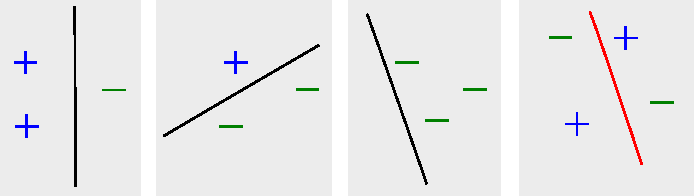
\includegraphics[width=1.0\textwidth]{thesis2/theory_PRML_shattering.pdf}
%	 \caption{A linear classifier in $\mathbb{R}^D$ can shatter $D+1$ points. Here, in the first 3 examples, a line in $\mathbb{R}^2$ is able to shatter 3 points. However, in the fourth example, it is unable to shatter 4 points.}
%	 \label{fig:shattering}
%	 \end{figure}
%
%\item \underline{VC dimension of NN classifier}. It has been shown by Kara\c{c}ali and Krim~\cite{2003_JNL_PRML_Karacali} that the VC dimension of the NN classifier is given by the number of reference points in the training set~\cite{2005_CNF_ML_Angiulli}. These reference points can be obtained from the codevectors of a VQ codebook, such as an RVQ codebook. For an RVQ codebook with $Q$ stages, and $M$ code-vectors per stage, there are $M^Q$ equivalent code-vectors. Moreover, the number of direct-sum code-vectors at the end of the $q$-th stage is $M^q$\footnote{This assumes that there are no null code-vectors, i.e. code-vectors in which all elements are 0.}. Therefore, the VC dimension of an RVQ nearest neighbor classifier in a variable-rate framework depends on how many stages and codevectors per stage are used. Changing these numbers can be used to change the VC dimension of the RVQ NN classifier, and hence its generalization ability.
%\end{enumerate}
%=========================
\section{Experiments}
%=========================
We use four datasets in $\mathbb{R}^{1089}$: (a) Uniform random variable, (c) Gaussian random variable, (c) Gauss-Markov random variable, and (d) images from the Dudek sequence. The reason for using $\mathbb{R}^{1089}$ is that our targets for all our tracking datasets are warped to a canonical size of 33-pixel height and 33-pixel width (33x33=1089). In all cases, we take 100 examples and split them up using an 80/20 rule, i.e. 80 training examples and 20 test examples. 10 cross-validation runs are used. In each cross-validation run, the training and test examples are picked randomly in the 80/20 ratio.
%Our goal is to examine the effects on training and test error of varying $q$, the number of stages in RVQ, while keeping $m$, the number of code-vectors per stage fixed. For this, we train an 8x4 RVQ (maximum q=8, m=4) using four different data distributions in $\mathbb{R}^{1089}$: (a) Dudek sequence, (b) Uniform random variable, (c) Gaussian random variable, and (d) Gauss-Markov random variable.
%=========================
\section{Results}
%=========================
Results for PCA, RVQp, RVQm and TSVQ are shown in Appendix~\ref{App:plots} as Figures~\ref{fig:PCA_results}, \ref{fig:RVQ_results_varyingP} \ref{fig:RVQ_results_varyingM} and \ref{fig:TSVQ_results} respectively.
We make the following observations from the results:
\begin{enumerate}
\item \textbf{Training error}. Training error is always less than test error, as expected. Also, for each of the algorithms individually, we observe,
\begin{itemize}
\item \underline{PCA}: Monotonic decrease with increasing $Q$. Training error becomes 0 when 80 eigenvectors are used, since there are 80 training examples.
\item \underline{RVQp}: Monotonic decrease with increasing $P$.
\item \underline{RVQm}: Can increase or decrease with increasing $M$, but slight variation.
\item \underline{TSVQ}: Monotonic decrease with increasing $P$.
\end{itemize}
\item \textbf{Test error}.
\begin{itemize}
\item \underline{Statistically independent data}: For the uniform and Gaussian random variables, test error for PCA and RVQp stays almost constant with increasing $Q$ and $P$ respectively. For RVQm and TSVQ, test error increases with increasing $P$. The reason is that PCA and RVQp use successive refinement when increasing $Q$ and $P$ respectively. Test error is therefore not expected to get better since it is not possible to better explain random data with increasing $Q$ and $P$.
On the other hand, RVQm and TSVQ control generalization ability with increasing $Q$, as discussed in an earlier report on VC dimension. Therefore, when the number of code-vectors increases, they tend to explain the training data well and are unable to explain the test data. For both RVQm and TSVQ, notice that when training error falls off sharply, test error increases sharply. Also, when training error drop is gradual, so is test error increase rate. This confirms over-generalization behavior. Also, RVQ increase or decrease rates are more gradual than TSVQ. And finally, the over-generalization for both RVQm and TSVQ is less pronounced with uniform random data than with Gaussian random data since there is more uncertainty in the latter distribution.
\item \underline{Statistically dependent data}: For the Gauss-Markov and Dudek cases, all 4 algorithms display decreasing test error with increasing $Q$ or $P$. The "knee" is visible in all cases.
\end{itemize}
\end{enumerate}
In general, the training and test errors for RVQ are less than TSVQ. This is due to the fact that RVQ has access to all data at every stage while designing codebooks, and can therefore better optimize stage code-vectors. In TSVQ, data is partitioned at every stage and can lead to data starvation.
Training error of PCA is in general better than RVQ. This is expected since PCA can achieve perfect reconstruction when $Q$ comes close to the number of training examples $N$, $N<<D$. Test errors however are comparable.
%\begin{enumerate}
%\item In all 4 cases, Also, for all cases, the test error decreases at a slower rate than test error as expected.
%
%\item For the Dudek sequence, we see that the test error decreases up till about 30 eigenvectors and then levels off. This means that it takes about 30 eigenvectors to capture most of the linear dependencies in this dataset. After the 30 eigenvector mark, the test error does not increase since the test vectors are very similar to the training set. This is what one would expect in a tracking scenario over short periods of time.
%\end{enumerate}
%In the following experiments, we keep $m$, the number of code-vectors per stage constant and vary $q$, the number of stages. We see that as stages increase, the training error tends to decrease and so does test error, a sign of increasing VC dimension.
%We make the following observations for RVQ:
%\begin{enumerate}
%\item Training and test error decreases monotonically.
%%\item dRMSE is lower than eRMSE since the decoder is subject to one constraint while the encoder is subject to two.
%\item Test error is always larger than training error.
%\item Highest test error is for monR as explained earlier.
%\item The highest rms error is for the Dudek sequence. This is expected since the signal amplitudes are larger.
%\item For the random data experiments, highest error is for the Gaussian random variable since it has the highest entropy. This is followed by the uniform random variable. The lowest error is for the Gauss-Markov random variable since RVQ is able to capture the statistical correlation in the data.
%\item For the Dudek experiment
%\begin{itemize}
%%\item The error levels out after about 4 stages telling us that by about q=4, we are able to explain the statistical correlations in the data.
%%\item RofE tends to further decrease in error after 5th stage telling us that the test snippet is a lot like the training snippet.
%%\item maxQ which is forced to go all the way tells us, as mentioned in~\cite{1996_JNL_AdvancesRVQ_Barnes}, that using more stages in %decoding will in many cases decrease rmse even if there are slight "bumps", i.e. increases in rmse along the way.
%\item monR, the greedy approach has highest rmse.
%\item The curve has the "knee" that one would expect with a classifier as one increases the DoF.
%\item At level 5, we see that there is clearly an increase in rms error which is why monR and nulE level out (monR exits but I continue showing its exit rmse), nulE rides out the wave and in the last stage is able to decrease rms error by another 0.0062.
%\item maxQ and RofE take the very small increases in rms error, since they're not greedy, and are rewarded with gains as they use more and more stages.
%\end{itemize}
%\item The reconstruction error for the Gaussian and uniform random variables is almost constant when adding stages since this cannot explain a test example that is statistically independent of the training data. We see the same behavior in PCA and TSVQ as well.
%\item The reconstruction error for the Gaussian and uniform random variables increases when adding more code-vectors per stage since this causes over-generalization.
%\item For the Gauss-Markov example, the statistical correlation is captured in about 3 stages when varying $M$. and 3 code-vectors per stage when varying $P$.
%\item Of the random variable experiments, the highest reconstruction errors are for Gaussian, uniform and Gauss-Markov random variables, as expected. The reason is that the Gaussian distribution has the highest entropy, followed by the uniform random variable, and then followed by the statistically correlated Gauss-Markov random variable.
%\end{enumerate}
%In these experiments, we see that as $q$, the number of stages increases, training error and test error decrease. This is as expected. However, we intend to do more experiments using cross-validation to gain more confidence in these results.
%
%These initial experiments appear to confirm the fact that RVQ has variable VC dimension. Whereas it is to be expected that increasing stages will decrease reconstruction error, both at design-time and run-time, ERM (empirical risk minimization) from statistical learning theory can be used as a justification for the number of stages $q$ that are used in a given classification or tracking scenario.
%We make the following observations for TSVQ:
%\begin{enumerate}
%\item For the binary balanced-tree TSVQ, test error and training error for the Dudek and Gauss-Markov cases decrease as expected with increasing stages.
%
%\item However, for the datasets in which there is no correlation, TSVQ test error increases monotonically. It appears that the TSVQ code-book is over-trained. Since the test data is quite different from the training data, test error starts to increase.
%\end{enumerate}
%=========================
\section{Conclusions}
%=========================
RVQ has 2 knobs, $P$ and $M$. In varying $P$, it acts like PCA in providing successive approximation. In varying $M$, it acts like TSVQ in changing its VC dimension, and therefore its generalization ability.
Given this flexibility, it is expected that RVQ will perform well in tracking experiments.
\newpage
\appendix
\section{Plots}
\label{App:plots}
The following pages contain plots for 4 experiments using PCA, RVQp, RVQm and TSVQ to measure rms errors for target reconstruction:
\begin{enumerate}
\item PCA: varying number of eigenvectors, $Q$.
\item RVQ: varying number of stages $P$ while holding the number of code-vectors per stage constant at $M=4$.
\item RVQ: varying number of code-vectors per stage while holding the number of stages constant at $P=8$.
\item TSVQ: varying number of stages $P$.
\end{enumerate}
%---------------------------------
\newpage
\subsection{PCA, varying number of eigenvectors $Q$}
%---------------------------------
\begin{figure}[h]
\subfigure[Uniform random variable $U\sim$ \texttt{[}0, 1\texttt{]} in $\mathbb{R}^{1089}$, 100 realizations.]{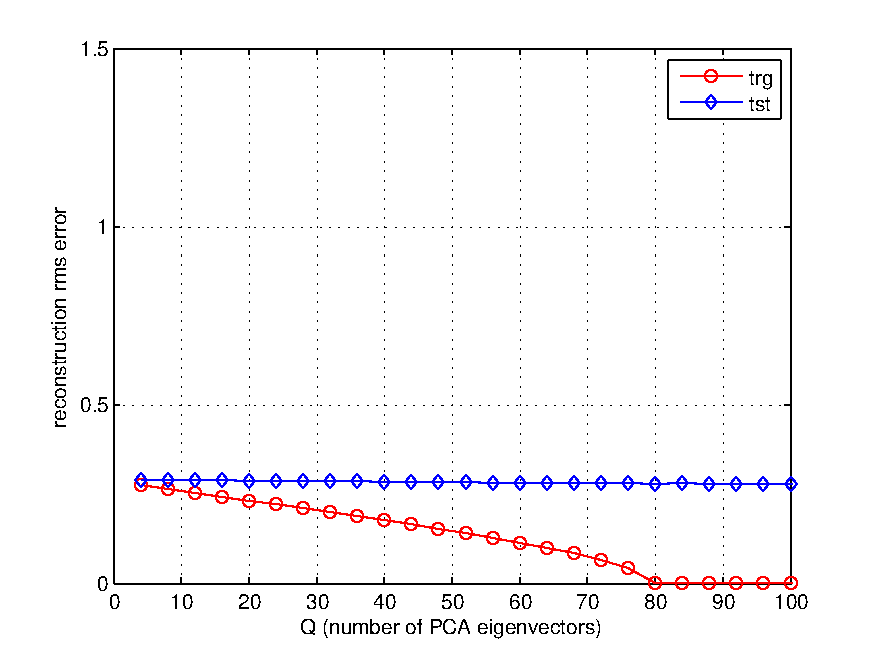
\includegraphics[width=0.45\textwidth]{thesis2/PCA_Uniform.pdf}}
\subfigure[Gaussian random variable $\mathcal{N}\sim$(0, 1) in $\mathbb{R}^{1089}$, 100 realizations.]{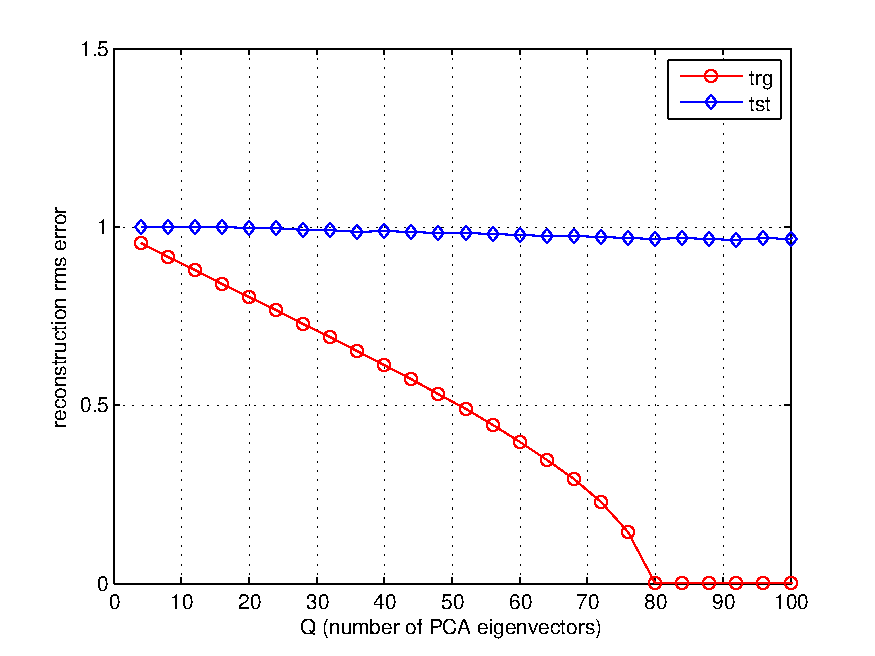
\includegraphics[width=0.45\textwidth]{thesis2/PCA_Gaussian.pdf}}
\subfigure[Gauss-Markov random variable $\mathcal{N}\sim$(0, 1) in $\mathbb{R}^{1089}$ with 0.9 correlation, 100 realizations.]{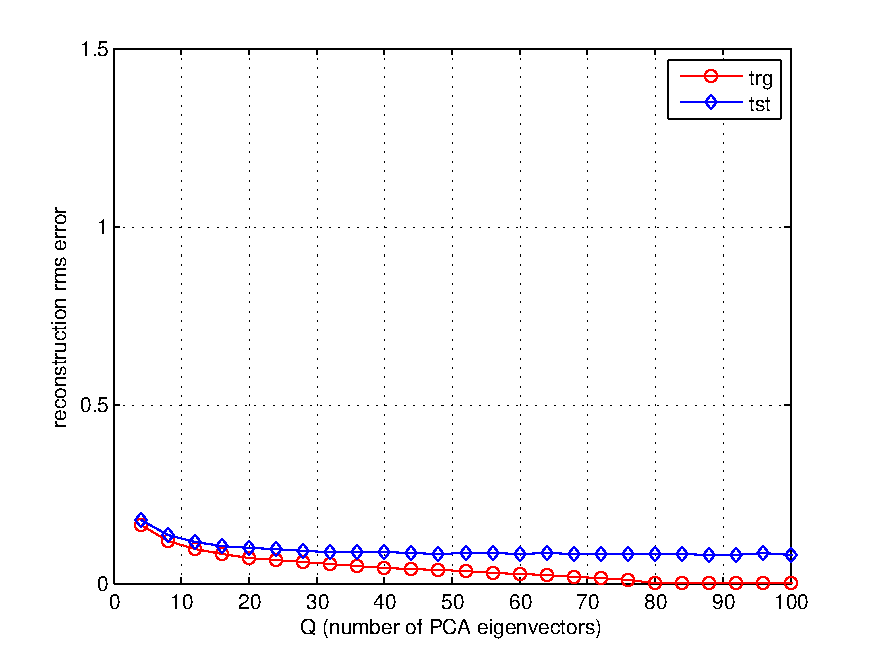
\includegraphics[width=0.45\textwidth]{thesis2/PCA_GaussMarkov.pdf}}\hspace{0.55in}
\subfigure[Dudek sequence, 33x33 ($\mathbb{R}^{1089}$) face snippets were extracted from the first 100 images.]{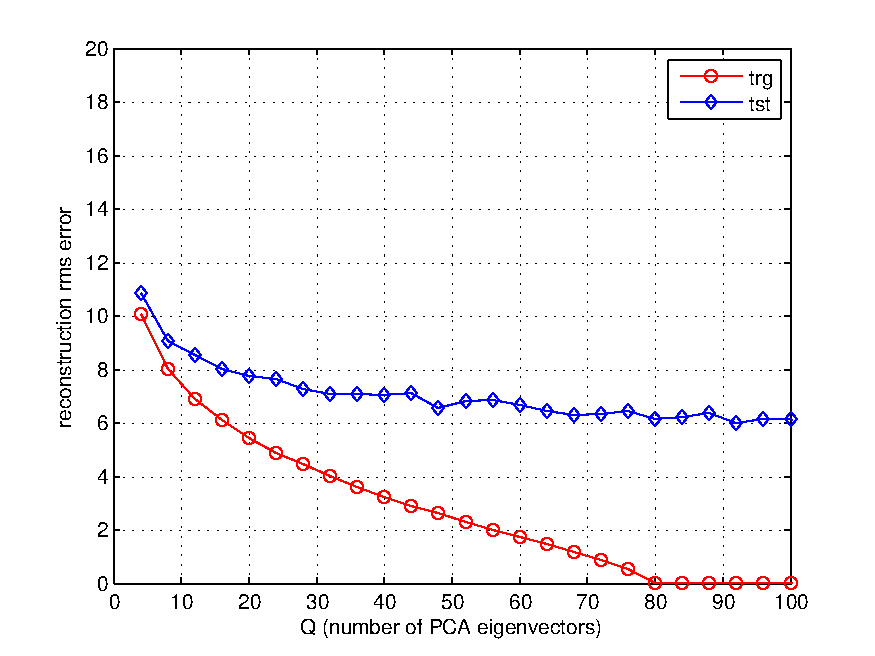
\includegraphics[width=0.45\textwidth]{thesis2/PCA_Dudek.pdf}}
\caption{PCA, 100 training examples in $\mathbb{R}^{1089}$ were used for each of these experiments. Results were averaged over 10 cross-validation runs. For each run, 20\% of the data, i.e., 20 examples were randomly picked for testing while the remaining 80 examples were used for training.}
\label{fig:PCA_results}
\end{figure}
%---------------------------------
\newpage
\subsection{RVQp, varying number of stages $P$}
%---------------------------------
\begin{figure}[h]
\subfigure[Uniform random variable $U\sim$ \texttt{[}0, 1\texttt{]} in $\mathbb{R}^{1089}$, 100 realizations.]
{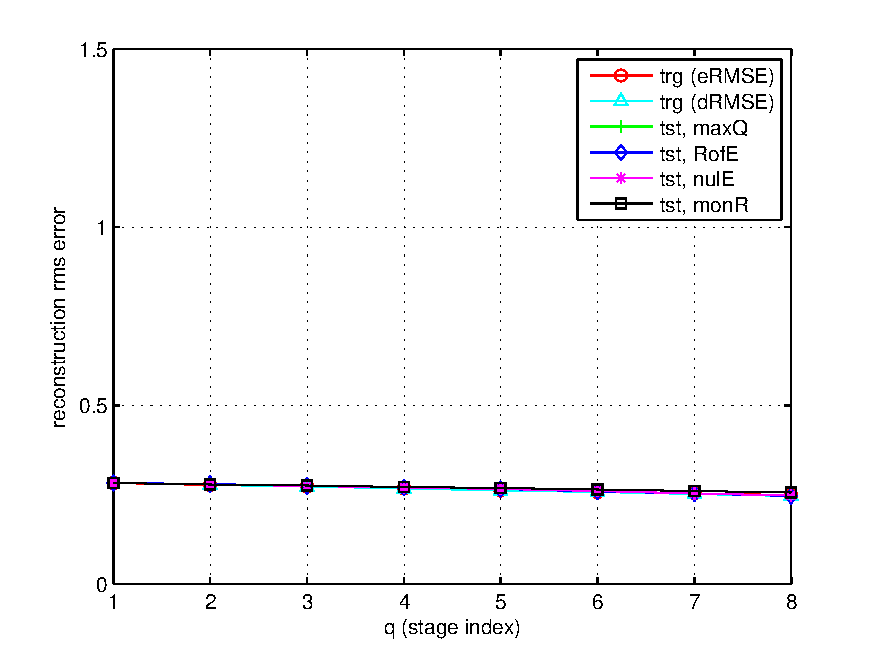
\includegraphics[width=0.45\textwidth]{thesis2/RVQ_8x4_Uniform.pdf}}
\subfigure[Gaussian random variable $\mathcal{N}\sim$(0, 1) in $\mathbb{R}^{1089}$, 100 realizations.]
{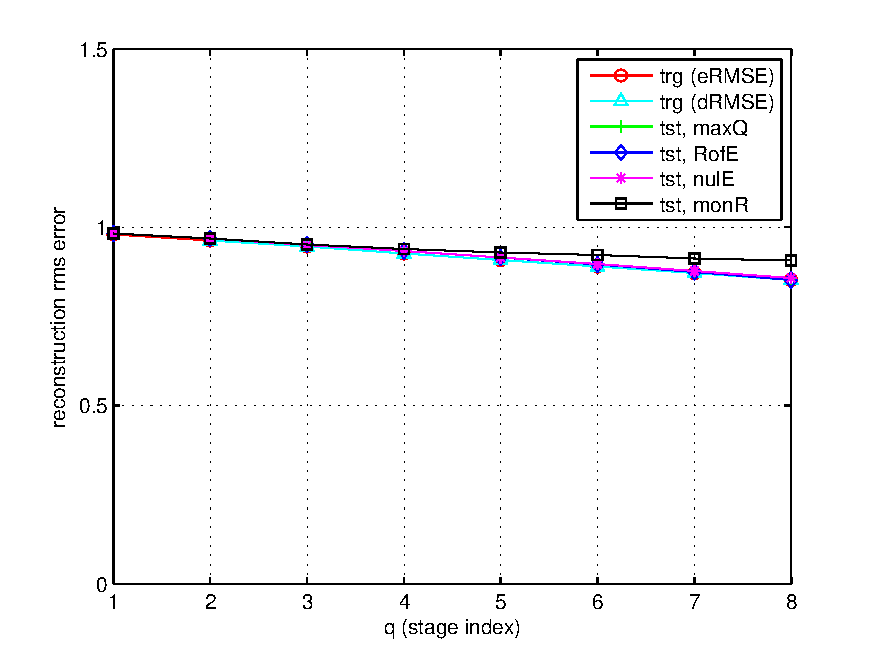
\includegraphics[width=0.45\textwidth]{thesis2/RVQ_8x4_Gaussian.pdf}}
\subfigure[Gauss-Markov random variable $\mathcal{N}\sim$(0, 1) in $\mathbb{R}^{1089}$ with 0.9 correlation, 100 realizations.]
{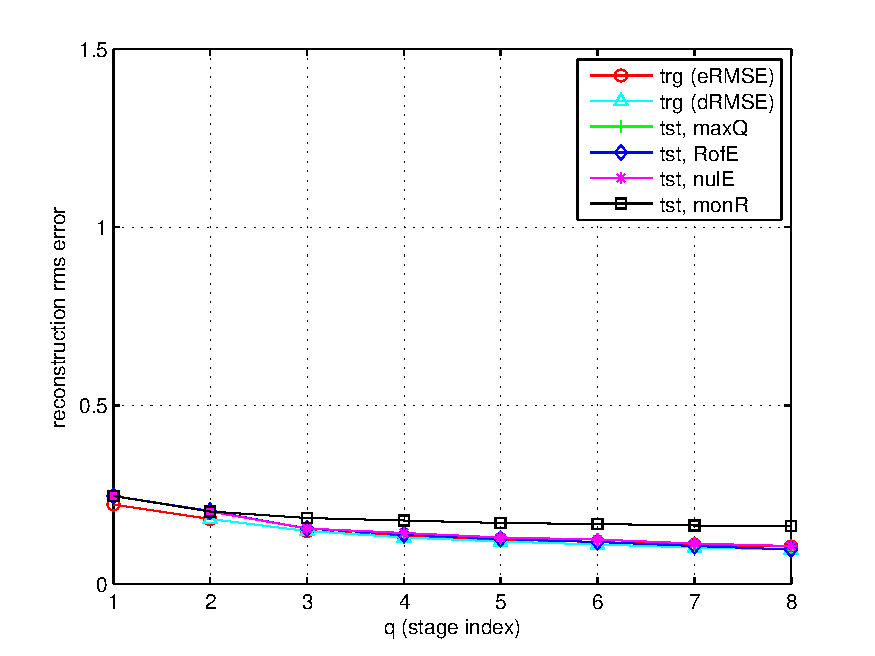
\includegraphics[width=0.45\textwidth]{thesis2/RVQ_8x4_GaussMarkov.pdf}}\hspace{0.55in}
\subfigure[Dudek sequence, 33x33 ($\mathbb{R}^{1089}$) face snippets were extracted from the first 100 images.]
{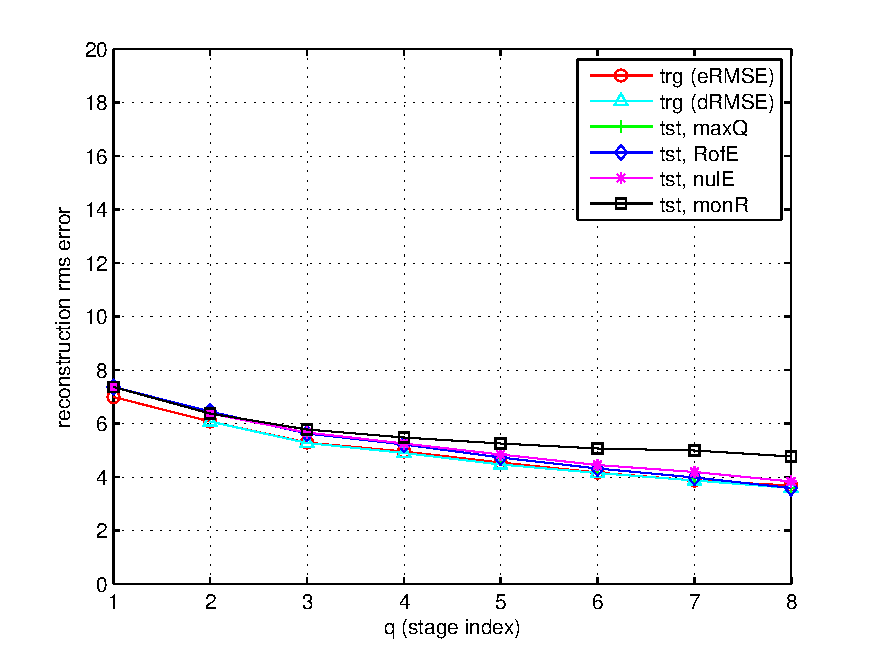
\includegraphics[width=0.45\textwidth]{thesis2/RVQ_8x4_Dudek.pdf}}
\caption{RVQp, varying number of stages $P$ with number of code-vectors per stage held constant at $M=4$. 100 training examples in $\mathbb{R}^{1089}$ were used for each of these experiments. A single test example in $\mathbb{R}^{1089}$ was reconstructed.}
\label{fig:RVQ_results_varyingP}
\end{figure}
%---------------------------------
\newpage
\subsection{RVQm, varying number of code-vectors per stage, $M$}
%---------------------------------
\begin{figure}[h]
\subfigure[Uniform random variable $U\sim$ \texttt{[}0, 1\texttt{]} in $\mathbb{R}^{1089}$, 100 realizations.]
{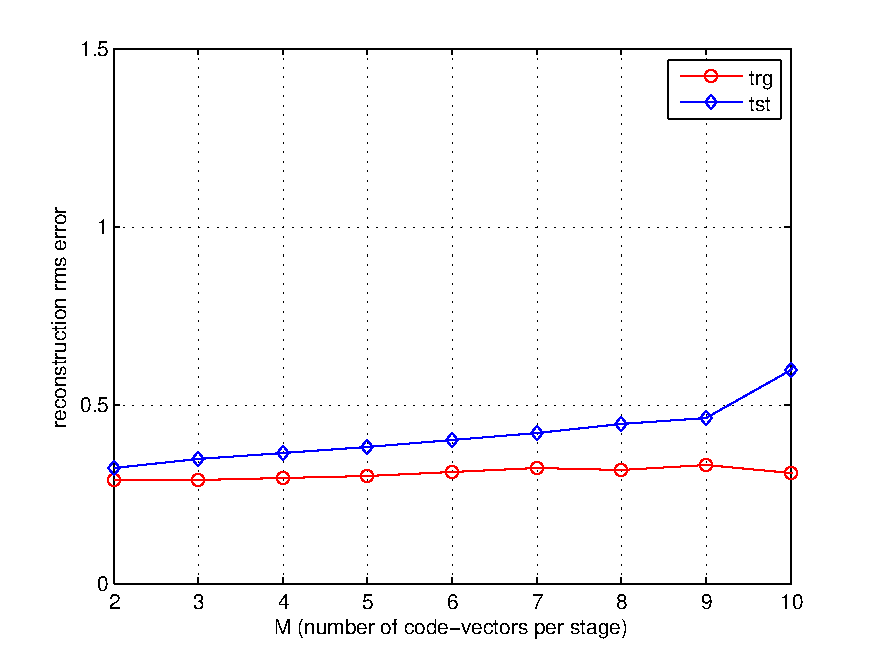
\includegraphics[width=0.45\textwidth]{thesis2/RVQ_uniform.pdf}}
\subfigure[Gaussian random variable $\mathcal{N}\sim$(0, 1) in $\mathbb{R}^{1089}$, 100 realizations.]
{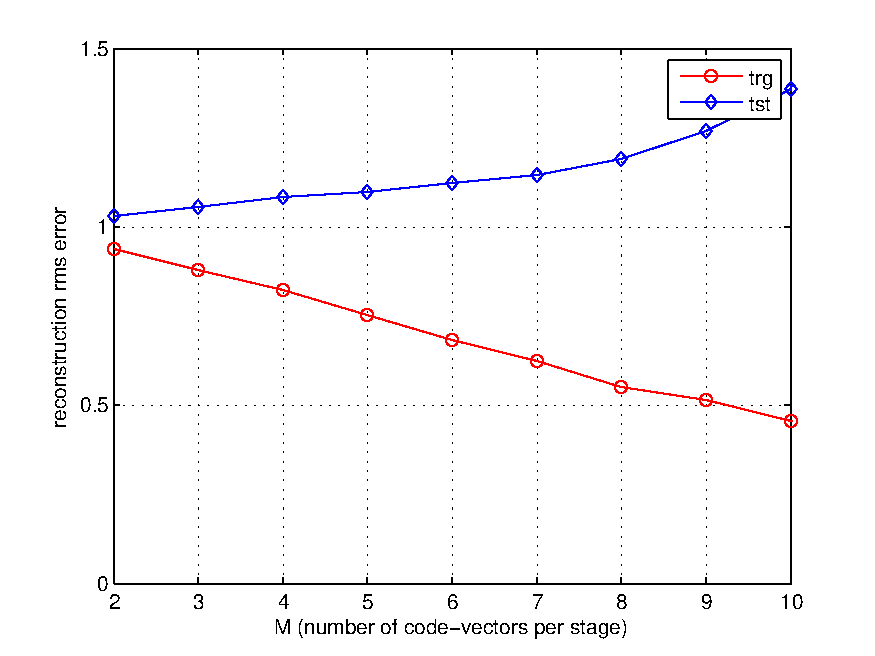
\includegraphics[width=0.45\textwidth]{thesis2/RVQ_Gaussian.pdf}}
\subfigure[Gauss-Markov random variable $\mathcal{N}\sim$(0, 1) in $\mathbb{R}^{1089}$ with 0.9 correlation, 100 realizations.]
{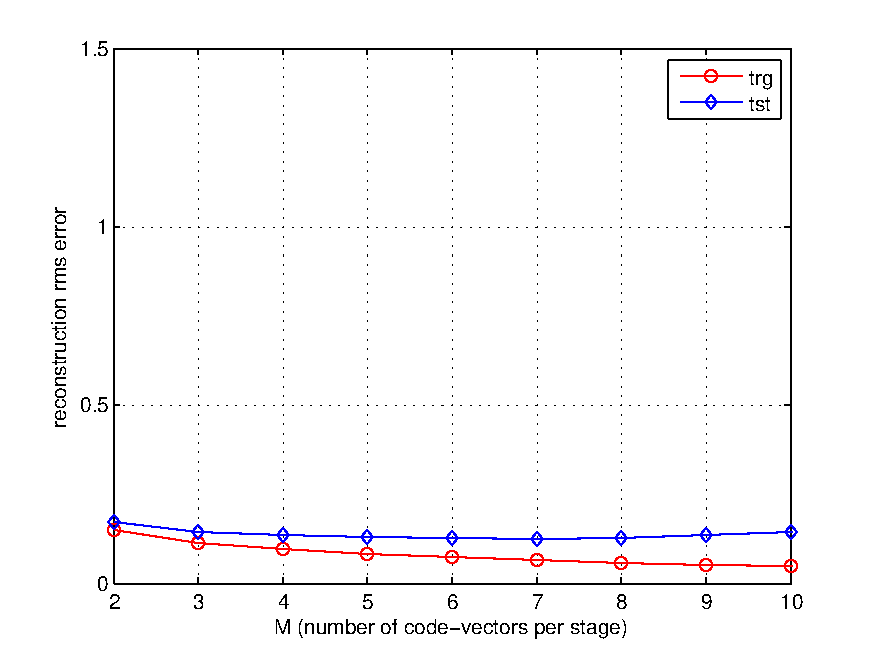
\includegraphics[width=0.45\textwidth]{thesis2/RVQ_GaussMarkov.pdf}}\hspace{0.55in}
\subfigure[Dudek sequence, 33x33 ($\mathbb{R}^{1089}$) face snippets were extracted from the first 100 images.]
{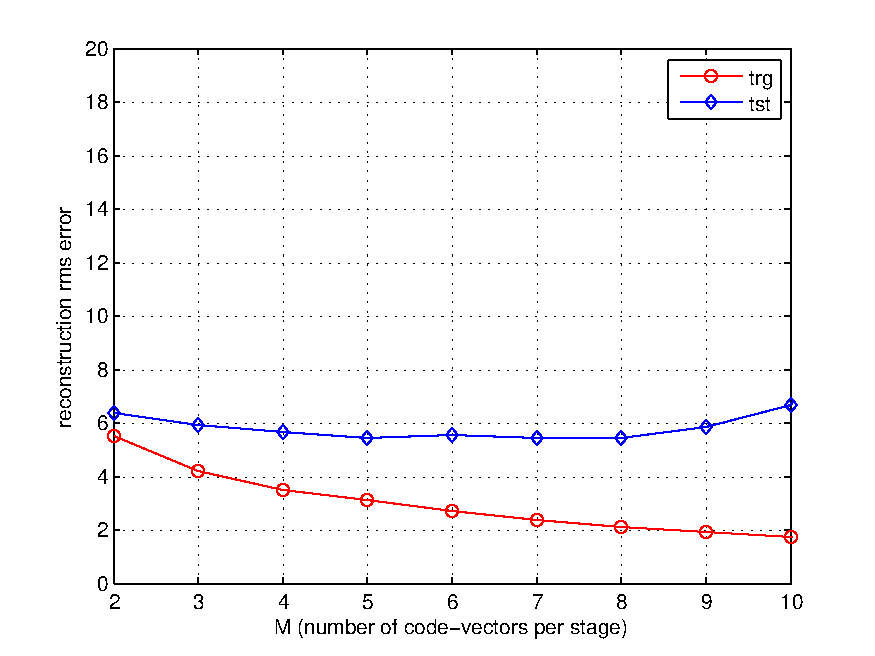
\includegraphics[width=0.45\textwidth]{thesis2/RVQ_Dudek.pdf}}
\caption{RVQm, experiments, varying number of code-vectors per stage $M$ with number of stages held constant at $P=8$. 100 training examples in $\mathbb{R}^{1089}$ were used for each of these experiments. Results were averaged over 10 cross-validation runs. For each run, 20\% of the data, i.e., 20 examples were randomly picked for testing while the remaining 80 examples were used for training.}
\label{fig:RVQ_results_varyingM}
\end{figure}
%---------------------------------
\newpage
\subsection{TSVQ, varying number of stages, $P$}
%---------------------------------
\begin{figure}[h]
\subfigure[Uniform random variable $U\sim$ \texttt{[}0, 1\texttt{]} in $\mathbb{R}^{1089}$, 100 realizations.]{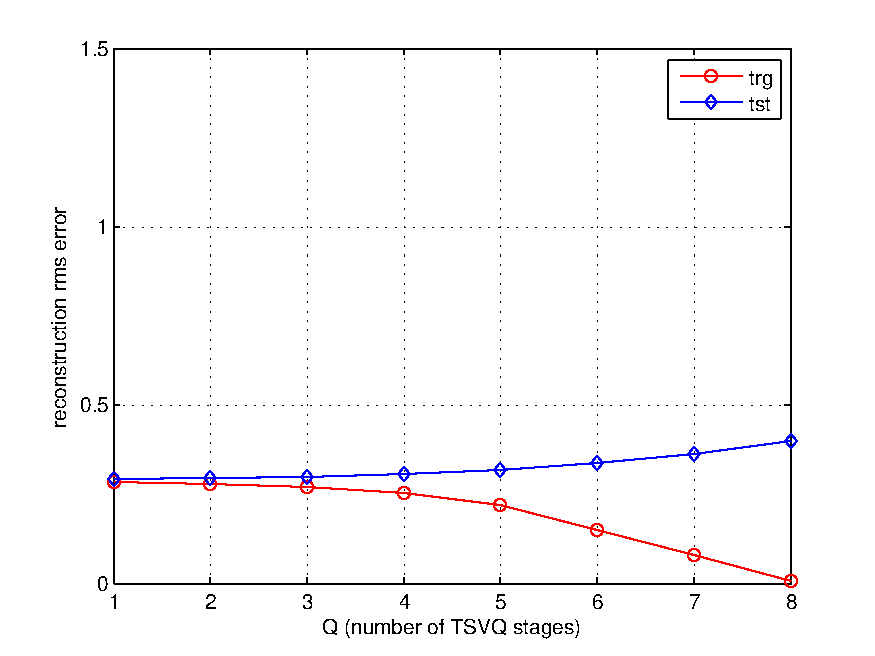
\includegraphics[width=0.45\textwidth]{thesis2/TSVQ_Uniform.pdf}}
\subfigure[Gaussian random variable $\mathcal{N}\sim$(0, 1) in $\mathbb{R}^{1089}$, 100 realizations.]{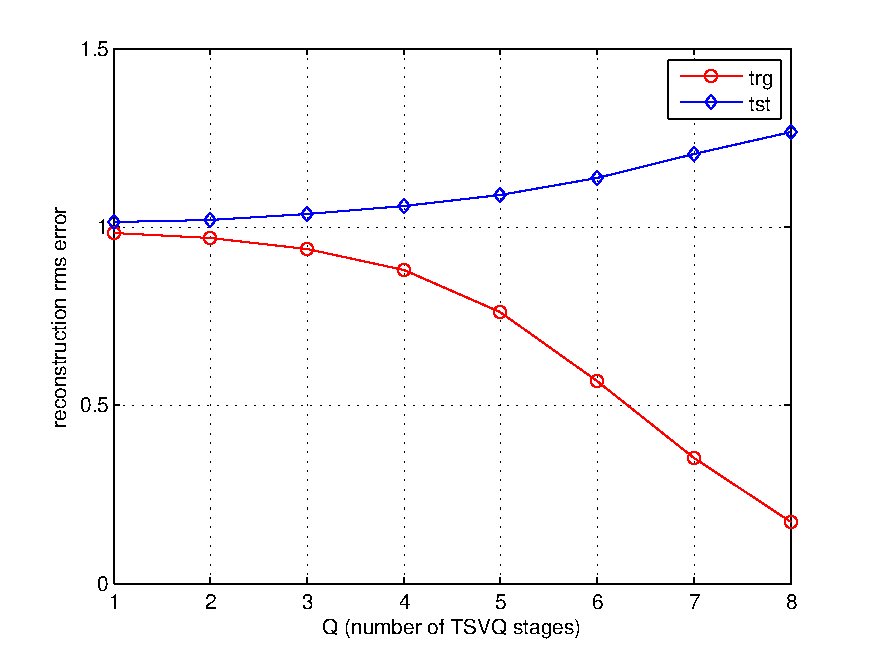
\includegraphics[width=0.45\textwidth]{thesis2/TSVQ_Gaussian.pdf}}
\subfigure[Gauss-Markov random variable $\mathcal{N}\sim$(0, 1) in $\mathbb{R}^{1089}$ with 0.9 correlation, 100 realizations.]{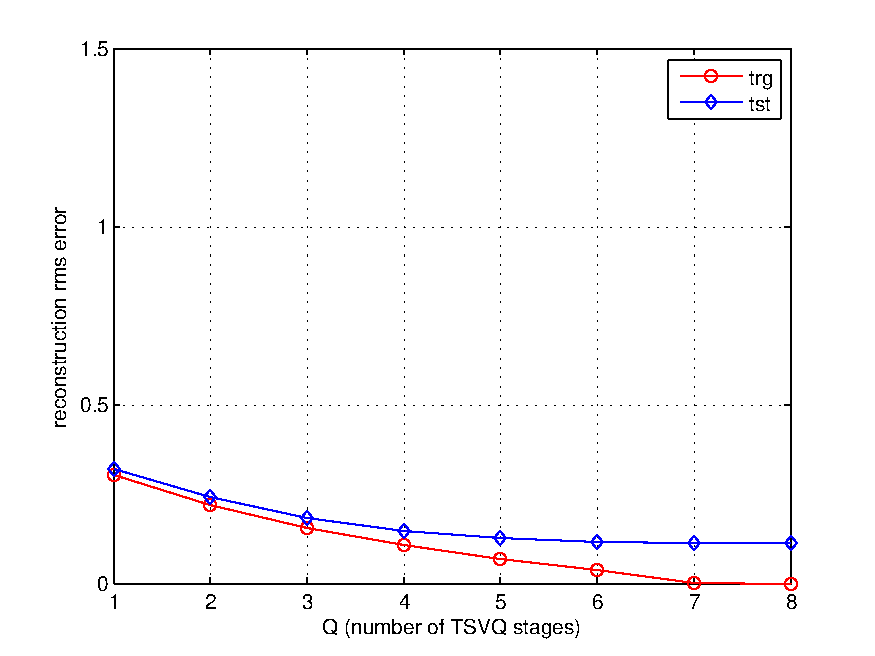
\includegraphics[width=0.45\textwidth]{thesis2/TSVQ_GaussMarkov.pdf}}\hspace{0.55in}
\subfigure[Dudek sequence, 33x33 ($\mathbb{R}^{1089}$) face snippets were extracted from the first 100 images.]{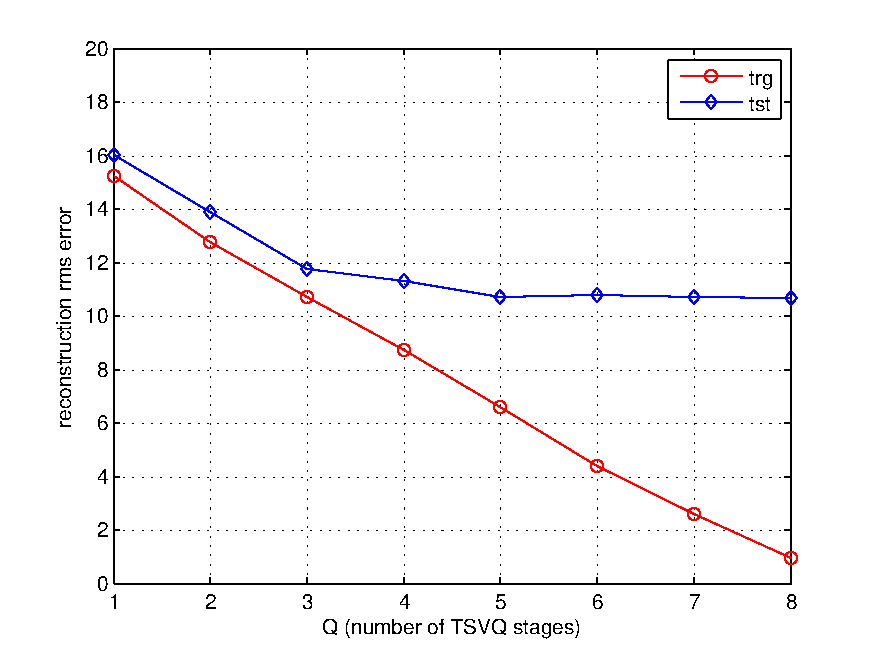
\includegraphics[width=0.45\textwidth]{thesis2/TSVQ_Dudek.pdf}}
\caption{TSVQ, 100 training examples in $\mathbb{R}^{1089}$ were used for each of these experiments. Results were averaged over 10 cross-validation runs. For each run, 20\% of the data, i.e., 20 examples were randomly picked for testing while the remaining 80 examples were used for training.}
\label{fig:TSVQ_results}
\end{figure}
\clearpage
\newpage
\normalsize
\bibliographystyle{ieee}
\bibliography{MyCitations}
\end{document}
%\subfigure[Dudek sequence, 33x33 ($\mathbb{R}^{1089}$) face snippets were extracted from the first 100 images. The ground truth affine parameters $\theta, \lambda_1, \lambda_2, t_x, t_y$ used to extract the snippets from the images were corrupted with zero-mean additive gaussian-noise (standard deviation 0.1) to simulate the effect of errors in tracking estimates.]{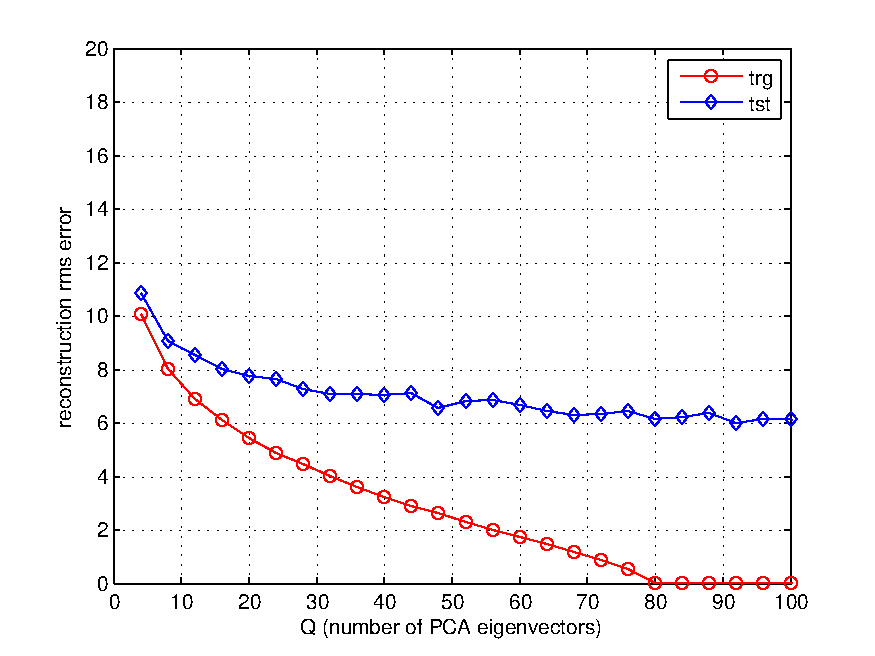
\includegraphics[width=0.45\textwidth]{thesis2/PCA_Dudek_noisy.pdf}}\hspace{0.2in}
%\subfigure[Dudek sequence, 33x33 ($\mathbb{R}^{1089}$) face snippets were extracted from the first 100 images. The ground truth affine parameters $\theta, \lambda_1, \lambda_2, t_x, t_y$ used to extract the snippets from the images were corrupted with zero-mean additive gaussian-noise (standard deviation 0.1) to simulate the effect of errors in tracking estimates.]{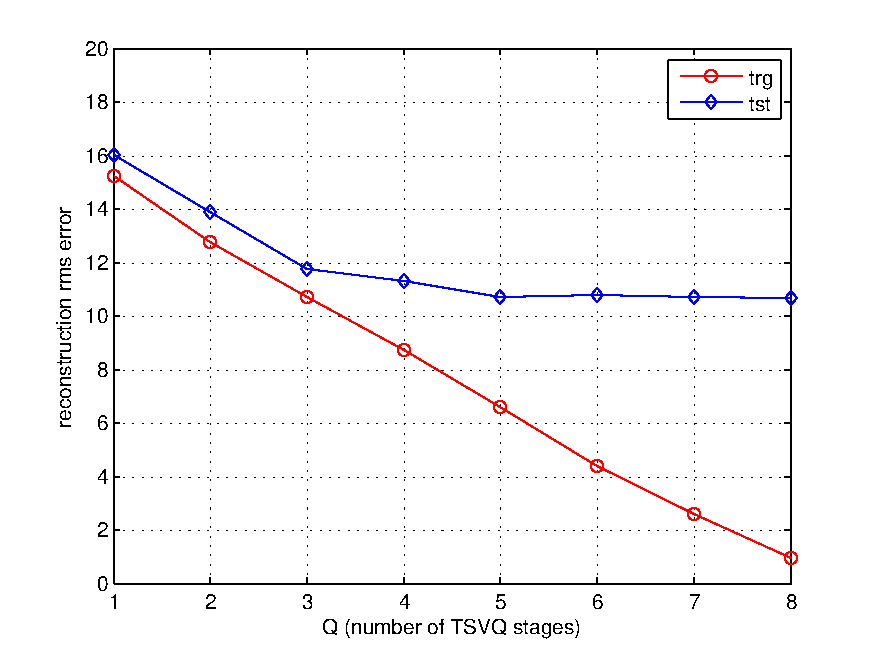
\includegraphics[width=0.45\textwidth]{thesis2/TSVQ_Dudek_noisy.pdf}}\hspace{0.2in}